\chapter{Langages et automates}

%Esperza et blondin automate sipser pour livres
Pour rappel : on a vu le \textbf{problème} suivant :

Etant donné un mot binaire, contient- il le facteur "101" ?
On est avec l'aplhabet $\Sigma = \{0,1\}$ et $\mathcal{L}_{101} = \{w\in \sigma^* | w \text{contient le facteur "101"}\}$
On peut réflechir à un algorithme pour déterminer si un mot appartient à $ \mathcal{L}_{101}$.

On veut donc trouver un algorithme pour reconnaitre (décider oui ou non en s'arretant ). Nous allons constuire un automate

\begin{definition}[informel]
    Un automate c'est une machine qui reconnait un langage ca va manger un mot lettre apres lettre et dira s'il est accepter pas.
\end{definition}
Pour notre problème on construit l'automate suivant : 

\begin{centering}


\tikzset{every picture/.style={line width=0.75pt}} %set default line width to 0.75pt        

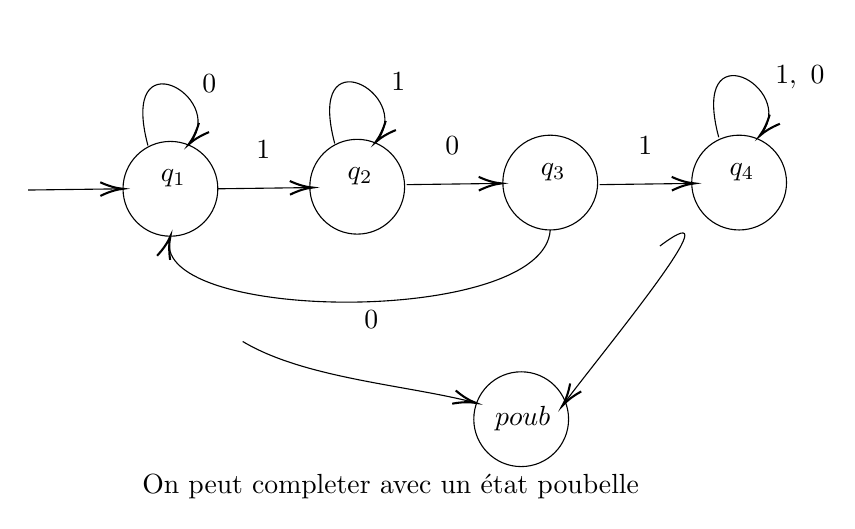
\begin{tikzpicture}[x=0.75pt,y=0.75pt,yscale=-1,xscale=1]
%uncomment if require: \path (0,300); %set diagram left start at 0, and has height of 300

%Shape: Circle [id:dp39159318436141544] 
\draw   (176,104.83) .. controls (176,92.22) and (186.22,82) .. (198.83,82) .. controls (211.44,82) and (221.67,92.22) .. (221.67,104.83) .. controls (221.67,117.44) and (211.44,127.67) .. (198.83,127.67) .. controls (186.22,127.67) and (176,117.44) .. (176,104.83) -- cycle ;
%Straight Lines [id:da23215206629411345] 
\draw    (130.33,105.43) -- (174,104.86) ;
\draw [shift={(176,104.83)}, rotate = 179.25] [color={rgb, 255:red, 0; green, 0; blue, 0 }  ][line width=0.75]    (10.93,-3.29) .. controls (6.95,-1.4) and (3.31,-0.3) .. (0,0) .. controls (3.31,0.3) and (6.95,1.4) .. (10.93,3.29)   ;
%Straight Lines [id:da6737208613248838] 
\draw    (221.67,104.83) -- (265.33,104.26) ;
\draw [shift={(267.33,104.23)}, rotate = 179.25] [color={rgb, 255:red, 0; green, 0; blue, 0 }  ][line width=0.75]    (10.93,-3.29) .. controls (6.95,-1.4) and (3.31,-0.3) .. (0,0) .. controls (3.31,0.3) and (6.95,1.4) .. (10.93,3.29)   ;
%Curve Lines [id:da7591834521750506] 
\draw    (188,84) .. controls (173.95,31.47) and (225.53,60.19) .. (208.78,82.07) ;
\draw [shift={(207.67,83.4)}, rotate = 312.27] [color={rgb, 255:red, 0; green, 0; blue, 0 }  ][line width=0.75]    (10.93,-3.29) .. controls (6.95,-1.4) and (3.31,-0.3) .. (0,0) .. controls (3.31,0.3) and (6.95,1.4) .. (10.93,3.29)   ;
%Shape: Circle [id:dp10471981573749756] 
\draw   (266,103.83) .. controls (266,91.22) and (276.22,81) .. (288.83,81) .. controls (301.44,81) and (311.67,91.22) .. (311.67,103.83) .. controls (311.67,116.44) and (301.44,126.67) .. (288.83,126.67) .. controls (276.22,126.67) and (266,116.44) .. (266,103.83) -- cycle ;
%Curve Lines [id:da770033043384433] 
\draw    (278,83) .. controls (263.95,30.47) and (315.53,59.19) .. (298.78,81.07) ;
\draw [shift={(297.67,82.4)}, rotate = 312.27] [color={rgb, 255:red, 0; green, 0; blue, 0 }  ][line width=0.75]    (10.93,-3.29) .. controls (6.95,-1.4) and (3.31,-0.3) .. (0,0) .. controls (3.31,0.3) and (6.95,1.4) .. (10.93,3.29)   ;
%Straight Lines [id:da8119244816386826] 
\draw    (312.67,102.83) -- (356.33,102.26) ;
\draw [shift={(358.33,102.23)}, rotate = 179.25] [color={rgb, 255:red, 0; green, 0; blue, 0 }  ][line width=0.75]    (10.93,-3.29) .. controls (6.95,-1.4) and (3.31,-0.3) .. (0,0) .. controls (3.31,0.3) and (6.95,1.4) .. (10.93,3.29)   ;
%Shape: Circle [id:dp9002917350521505] 
\draw   (359,101.83) .. controls (359,89.22) and (369.22,79) .. (381.83,79) .. controls (394.44,79) and (404.67,89.22) .. (404.67,101.83) .. controls (404.67,114.44) and (394.44,124.67) .. (381.83,124.67) .. controls (369.22,124.67) and (359,114.44) .. (359,101.83) -- cycle ;
%Curve Lines [id:da8427815305530494] 
\draw    (381.83,124.67) .. controls (378.88,170.96) and (191.42,169.46) .. (198.38,129.52) ;
\draw [shift={(198.83,127.67)}, rotate = 107.51] [color={rgb, 255:red, 0; green, 0; blue, 0 }  ][line width=0.75]    (10.93,-3.29) .. controls (6.95,-1.4) and (3.31,-0.3) .. (0,0) .. controls (3.31,0.3) and (6.95,1.4) .. (10.93,3.29)   ;
%Straight Lines [id:da9519294285068559] 
\draw    (405.67,102.83) -- (449.33,102.26) ;
\draw [shift={(451.33,102.23)}, rotate = 179.25] [color={rgb, 255:red, 0; green, 0; blue, 0 }  ][line width=0.75]    (10.93,-3.29) .. controls (6.95,-1.4) and (3.31,-0.3) .. (0,0) .. controls (3.31,0.3) and (6.95,1.4) .. (10.93,3.29)   ;
%Shape: Circle [id:dp11252058259290443] 
\draw   (450,101.83) .. controls (450,89.22) and (460.22,79) .. (472.83,79) .. controls (485.44,79) and (495.67,89.22) .. (495.67,101.83) .. controls (495.67,114.44) and (485.44,124.67) .. (472.83,124.67) .. controls (460.22,124.67) and (450,114.44) .. (450,101.83) -- cycle ;
%Curve Lines [id:da9970488655619414] 
\draw    (463,80) .. controls (448.95,27.47) and (500.53,56.19) .. (483.78,78.07) ;
\draw [shift={(482.67,79.4)}, rotate = 312.27] [color={rgb, 255:red, 0; green, 0; blue, 0 }  ][line width=0.75]    (10.93,-3.29) .. controls (6.95,-1.4) and (3.31,-0.3) .. (0,0) .. controls (3.31,0.3) and (6.95,1.4) .. (10.93,3.29)   ;
%Curve Lines [id:da05531269471522049] 
\draw    (434.67,132.4) .. controls (473.87,103) and (406.14,184.43) .. (388.67,208.03) ;
\draw [shift={(387.67,209.4)}, rotate = 305.95] [color={rgb, 255:red, 0; green, 0; blue, 0 }  ][line width=0.75]    (10.93,-3.29) .. controls (6.95,-1.4) and (3.31,-0.3) .. (0,0) .. controls (3.31,0.3) and (6.95,1.4) .. (10.93,3.29)   ;
%Curve Lines [id:da0594437607240863] 
\draw    (233.67,178.4) .. controls (263.22,196.13) and (312.17,199.31) .. (344.53,207.62) ;
\draw [shift={(346,208)}, rotate = 194.89] [color={rgb, 255:red, 0; green, 0; blue, 0 }  ][line width=0.75]    (10.93,-3.29) .. controls (6.95,-1.4) and (3.31,-0.3) .. (0,0) .. controls (3.31,0.3) and (6.95,1.4) .. (10.93,3.29)   ;
%Shape: Circle [id:dp45992039591403555] 
\draw   (345,215.83) .. controls (345,203.22) and (355.22,193) .. (367.83,193) .. controls (380.44,193) and (390.67,203.22) .. (390.67,215.83) .. controls (390.67,228.44) and (380.44,238.67) .. (367.83,238.67) .. controls (355.22,238.67) and (345,228.44) .. (345,215.83) -- cycle ;

% Text Node
\draw (193,94.4) node [anchor=north west][inner sep=0.75pt]    {$q_{1}$};
% Text Node
\draw (213,48.4) node [anchor=north west][inner sep=0.75pt]    {$0$};
% Text Node
\draw (239,80.4) node [anchor=north west][inner sep=0.75pt]    {$1$};
% Text Node
\draw (283,93.4) node [anchor=north west][inner sep=0.75pt]    {$q_{2}$};
% Text Node
\draw (304,47.4) node [anchor=north west][inner sep=0.75pt]    {$1$};
% Text Node
\draw (330,78.4) node [anchor=north west][inner sep=0.75pt]    {$0$};
% Text Node
\draw (376,91.4) node [anchor=north west][inner sep=0.75pt]    {$q_{3}$};
% Text Node
\draw (291,162.4) node [anchor=north west][inner sep=0.75pt]    {$0$};
% Text Node
\draw (423,78.4) node [anchor=north west][inner sep=0.75pt]    {$1$};
% Text Node
\draw (467,91.4) node [anchor=north west][inner sep=0.75pt]    {$q_{4}$};
% Text Node
\draw (489,44.4) node [anchor=north west][inner sep=0.75pt]    {$1,\ 0$};
% Text Node
\draw (354,208.4) node [anchor=north west][inner sep=0.75pt]    {$poub$};
% Text Node
\draw (184,241) node [anchor=north west][inner sep=0.75pt]   [align=left] {On peut completer avec un état poubelle};


\end{tikzpicture}

\end{centering}

On peut tester l'automate sur différents mots et vérifier si l'état final est $q_4$ qui est acceptant.

\begin{remarque}
On peut remarquer que $w_1= 11$ et $w_2= 0001$ finissent sur le même état et en fait on verra qu'ils peuvent être vus comme équivalent en terme de continuiation qu'on verra plus tard.
\end{remarque}

En fait, un automate est $\mathcal{L}(\mathcal{A})\subseteq \Sigma^*$ qui prend $w\in \Sigma^*$ et qui accepte si $w\in \mathcal{L}(\mathcal{A})$ et rejette sinon.
